%----------------------------------------------------------------------------
\chapter{Implementation}
\label{cha:implementation}
%----------------------------------------------------------------------------

At the end of the design step it is clearly visible, what advantages the investigated technologies and tools have. The implementation of the created testing framework will be represented grouped by the model based testing process phases as earlier.

\begin{figure}[htp]
\centering
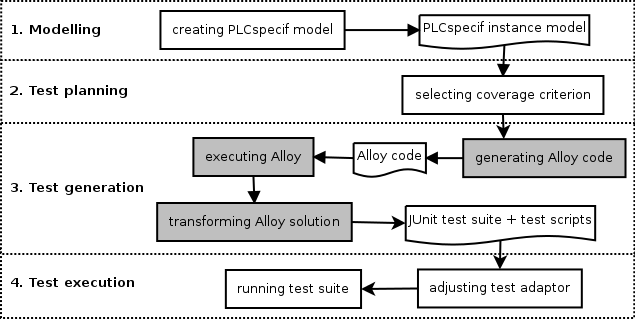
\includegraphics[scale=0.6]{figures/implementation_usage}
\caption{Usage of the test generator framework}
\label{fig:implementation_usage}
\end{figure}

Figure~\ref{fig:implementation_usage} demonstrates the usage of the testing framework. The manual operations are noted with white rectangles, the automatically executed operations are in grey rectangles. Outputs of the operations are represented with document symbols.

\begin{description}
	\item[1. Modelling] First the instance model have to be created with the default PLCspecif model editor generated by the Eclipse Modeling Framework.
	\item[2. Test planning]
	\item[3. Test generation] The next step is to create Alloy code, that can produce the test cases. The required informations can be extracted from the previously created PLCspecif model, and so the desired Alloy code can be generated automatically. This generation was solved with Acceleo, which is a model to text transforming tool as part of the Eclipse Modeling Tools.
	
	The generated Alloy code will be demonstrated with an example (see Figure~\ref{fig:alloy_statemachine}). The static part of the generated Alloy code can be see on Listing~\ref{lst:alloy_static}.

\begin{figure}[htp]
\centering
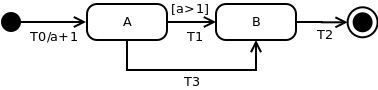
\includegraphics[scale=0.5]{figures/alloy_statemachine}
\caption{Example state machine with guard}
\label{fig:alloy_statemachine}
\end{figure}

The basic state machine element's (system, states, transitions) are between line number 4-7. The next section (line number 9-18.) describes the structure of a basic test case. One test case consists of several steps. The only given fact (line number 20-27.) defines the connection between a test case and the state machine. The predicate \texttt{inheritSystem} is a utility method, that can be used to inherit extended state variables from previous states. Predicates \texttt{transition\_coverage} and \texttt{state\_coverage} define transition and state coverage criteria accordingly. These predicates can be executed using the \texttt{run} statement used in line number 38.

\begin{lstlisting}[label={lst:alloy_static}, caption=Test suite generator Alloy code,breaklines=true]

\end{lstlisting}

The dynamic part of the Alloy code, generated from the instance model can be see on Listing~\ref{lst:alloy_dynamic}. The code starts with the initialization of the SUT. The structure was defined in a signature, while the initial state of the SUT needs to define in a predicate. The rest of the code describes the other parts of the state machine: the states (\texttt{A}, \texttt{B}), the transitions (\texttt{T0}, \texttt{T1}, \texttt{T2}, \texttt{T3}), the events (\texttt{E0}) and the guards (\texttt{G0}).

\begin{lstlisting}[label={lst:alloy_dynamic}, caption=Dynamically generated Alloy codes,breaklines=true]

\end{lstlisting}

\begin{figure}[htp]
\centering
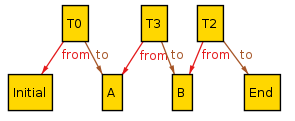
\includegraphics[scale=0.5]{figures/alloy_statecoverage}
\caption{Example test case generated from state machine in Figure~\ref{fig:alloy_statemachine}}
\label{fig:alloy_statecoverage}
\end{figure}

The above Alloy code generates test cases with state coverage guaranteed and the resulted test case is on Figure~\ref{fig:alloy_statecoverage} considering the previously defined state machine. As we can see the transition \texttt{T1}, having an unsatisfiable guard, is left out from the test case, and the generated test case satisfies all the requirements.

	The generated Alloy code guarantees state and transition coverages. To create the Alloy code, we need to know the name of states, transitions, their relationship, the guards and the initial state of the SUT. From these information will be the necessary Alloy signatures and predicates generated.
	\item[4. Test execution] The generated Alloy code can be executed with Alloy Analyzer to get the test suite with all the test cases.
\end{description}
% chapter implementation (end)